\documentclass[a4paper,12pt]{report}

\usepackage[utf8]{inputenc}
\usepackage[T1]{fontenc}
\usepackage[brazil]{babel}

\usepackage[titletoc]{appendix}
\usepackage{amsmath}
\usepackage{amsfonts}
\usepackage{amssymb}
\usepackage{amsthm}
\usepackage{setspace}
\usepackage{float}
\usepackage{mathrsfs}

\usepackage{listings}
\usepackage{fancybox}
\usepackage{hyperref}

\usepackage{indentfirst}
\usepackage[normalem]{ulem}
\usepackage{enumerate}

\usepackage{graphicx}
\usepackage{tikz, tkz-fct}
\usepackage{pgfplots}

\usepackage{geometry}
\geometry{
	a4paper,
	%total={170mm,257mm},
	left=3cm,
	right=3cm,
	top=3cm,
	bottom=3cm,
	includefoot}


\bibliographystyle{plain}

\newenvironment{psmallmatrix}
{\left(\begin{smallmatrix}}
	{\end{smallmatrix}\right)}

%\newtheorem{theorem}{Teorema}[section]
%\newtheorem{Defini}{Definição}[section]
\newtheorem{proposition}{Proposição}[section]
\newtheorem{observation}{Observação}[section]
%\newtheorem{Exemplo}{Exemplo}[section]
%\newtheorem{Teo}{Teorema}[chapter]
%\newtheorem{lema}[Teo]{Lema}

\newtheorem{Defini}{\bf Definição}
\newtheorem{Proposi}{\bf Proposição}
\newtheorem{Lema}{\bf Lema}
\newtheorem{Teo}{\bf Teorema}
\newtheorem{Coro}{\bf Corolário}
\newtheorem{Obs}{\bf Observação}
\newtheorem{Exemplo}{\bf Exemplo}


%%%%%%%%%%%%%%%%%%%%%%%%%%%%%%


\begin{document}
	
	
	
	\thispagestyle{empty}
	
	\begin{center}
		
		UNIVERSIDADE FEDERAL DO AMAZONAS\\
		INSTITUTO DE CIÊNCIAS EXATAS\\
		DEPARTAMENTO DE MATEMÁTICA
		
		\vspace{5 cm}
		\bf{DIEGO PAIVA TORRES}\\
		
		\vspace{5 cm}
		\begin{center}
			\Large {\bf {TÍTULO DO TRABALHO}}
		\end{center}
		
		
		\vspace{7cm}
		
		MANAUS - AM\\
		2026
	\end{center}
	
	\thispagestyle{empty}
	
	\newpage
	
	%%%%%%%%%%%%%%%%%%%%%%%%%%%%%%%%%%%%%	
	
	\thispagestyle{empty}
	
	\begin{center}
		\bf{DIEGO PAIVA TORRES} \vspace{7cm}\\
		
		\Large {\bf {TÍTULO DO TRABALHO}} \vspace{3cm}\\
	\end{center}
	
	\begin{flushright}
		\begin{minipage}[10cm]{8.5cm}
			{\footnotesize
				Trabalho de Conclusão de Curso apresentado ao Departamento de Matemática da Universidade Federal do Amazonas, como requisito para a obtenção do  título de Bacharel em Matemática Pura e Aplicada.\\ 
			}
		\end{minipage}
	\end{flushright}
	\vspace{1cm}
	
	\begin{center}
		{\bf Orientador:} Prof. Dr. Dimas Morera Martinez
	\end{center}
	
	
	
	\vspace{4cm}
	\begin{center}
		MANAUS-AM\\ 2026
	\end{center}
	\newpage
	%%%%%%%%%%%%%%%%%%%%%%%%%%%%%%%%
	
	\thispagestyle{empty}
	\begin{center}
		{\textbf{TERMO DE APROVAÇÃO}} 	
	\end{center}
	
	\vspace{1cm}
	
	\textbf{ACADÊMICA}: Diego Paiva Torres.\\
	
	\textbf{ÁREA DE CONCENTRAÇÃO}: Matemática Pura e Aplicada.\\
	
	\textbf{LINHA DE PESQUISA}: Processamento de Imagens.\\
	
	\textbf{GRADUAÇÃO EM MATEMÁTICA PURA E APLICADA}: Habilitação em Bacharelado.\\
	
	\textbf{TÍTULO DO TRABALHO DE CONCLUSÃO DE CURSO}: Título do Trabalho. \\
	
	\textbf{ORIENTADOR}: Prof. Dr. Dimas Morera Martinez.\\
	
	\vspace{5cm}
	
	\begin{center}
		
		
		
		-----------------------------------------------------------------------------
		
		Prof. Dr.  Dimas Morera Martinez (Orientador)
		
		Universidade Federal do Amazonas (UFAM) - DM
		\vskip 1 cm
		
		-----------------------------------------------------------------------------
		
		Prof. Dr. Banca 1
		
		Universidade Federal do Amazonas (UFAM) - DM
		\vskip 1 cm
		
		-----------------------------------------------------------------------------
		
		Prof. Dr. Banca 2
		
		Universidade Federal do Amazonas (UFAM) - DM
	\end{center}
	
	
	
	\newpage
	
	%%%%%%%%%%%%%%%%%%%%%%%%%%%%%%%%%%%%%
	\thispagestyle{empty}
	\vfill
	\begin{center}
		\textit{À minha família.}
	\end{center}
	\vfill
	
	\newpage
	%%%%%%%%%%%%%%%%%%%%%%%%%%%%%%%%%%%%%%%%%%%
	
	\chapter*{\centering{Agradecimentos}}
	
	
	
	\thispagestyle{empty}
	\newpage
	
	%%%%%%%%%%%%%%%%%%%%%%%%%%%%%%%%%%%%%
	
	\chapter*{\centering Resumo}
	
	
	
	
	\thispagestyle{empty} 
	
	\newpage
	
	\chapter*{\centering Abstract}
	
	
	
	
	\thispagestyle{empty} 
	\newpage
	%%%%%%%%%%%%%%%%%%%%%%%%%%%%%%%%%%%%%%%
	%SUMARIO%
	%%%%%%%%%%%%%%%%%%%%%%%%%%%%%%%%%%%%%%
	
	
	\begin{titlepage}
		\tableofcontents
		\thispagestyle{empty}
	\end{titlepage}
	
	\newpage
	
	%%%%%%%%%%%%%%%%%%%%%%%%%%%%%%%%%%%%%
	
	\chapter*{Introdução}
	\addcontentsline{toc}{chapter}{Introdução}
	
	
	\newpage
	
	%%%%%%%%%%%%%%%%%%%%%%%%%%%%%%%%%%%%%%
	
	\chapter{Definições Básicas}

No estudo do processamento digital de imagens sob a perspectiva da matemática pura e aplicada, a primeira etapa fundamental consiste na formalização rigorosa do conceito de imagem contínua e na análise dos processos de discretização necessários para a sua representação computacional.

Neste capítulo, formalizaremos o modelo contínuo de formação de imagem baseado nas componentes físicas de iluminação e refletância, a discretização do domínio espacial através do processo de \textbf{amostragem}, e a discretização do contradomínio de intensidades através da \textbf{quantização}. Por fim, introduziremos a representação matricial de imagens digitais, os métodos de interpolação e a topologia discreta no reticulado.

\section{Conceito Matemático de Imagem Contínua}

Do ponto de vista matemático, uma imagem monocromática estática pode ser modelada como uma função de duas variáveis reais cujo contradomínio representa os níveis de intensidade luminosa ou escala de cinza.

\begin{Defini}[Imagem Monocromática Contínua]
Seja $U = [a,b] \times [c,d] \subset \mathbb{R}^2$ um retângulo compacto e conexo, denominado \textbf{suporte espacial} ou \textbf{domínio da imagem}. Uma \textbf{imagem monocromática contínua} é uma função mensurável $f: U \to V$, onde $V = [L_{\min}, L_{\max}] \subset \mathbb{R}^+$ ($0 \le L_{\min} < L_{\max} < \infty$) representa a \textbf{escala de intensidades} ou \textbf{escala de cinza}. Para cada ponto de coordenadas $(x,y) \in U$, o valor $f(x,y) \in V$ denota a intensidade luminosa da imagem nesse ponto.
\end{Defini}

Por convenção normalizada, quando $V = [0, 1]$, a intensidade $f(x,y) = 0$ representa a ausência total de luz (preto), enquanto $f(x,y) = 1$ representa a intensidade máxima (branco). Níveis intermediários $0 < f(x,y) < 1$ correspondem a variações graduais de cinza.

A Figura \ref{fig:arara_cinza} ilustra um exemplo de fotografia monocromática em escala de cinza.

\begin{figure}[H]
	\centering
	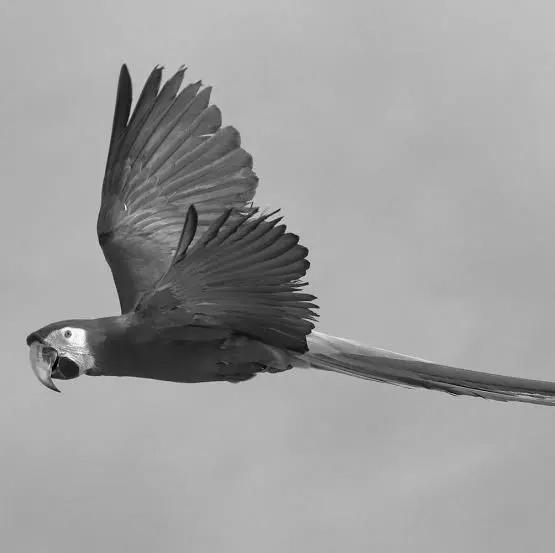
\includegraphics[width=0.5\linewidth]{arara_cinza.jpg}
	\caption{Exemplo de imagem monocromática em escala de cinza.}
	\label{fig:arara_cinza}
\end{figure}

\subsection{Modelo Físico de Formação de Imagem}

Fisicamente, a intensidade luminosa capturada por um dispositivo em uma cena tridimensional decorre da interação entre a iluminação proveniente da fonte emissora e a refletância dos objetos presentes na cena.

\begin{Defini}[Modelo de Iluminação-Refletância]
A função de intensidade de uma imagem contínua $f(x,y)$ pode ser decomposta como o produto de duas funções escalares positivas:
\begin{equation}
f(x,y) = i(x,y) \cdot r(x,y), \quad \forall (x,y) \in U
\end{equation}
onde:
\begin{enumerate}[(i)]
	\item $i: U \to (0, \infty)$ é a \textbf{função de iluminação}, que mede a quantidade de luz incidente sobre a cena no ponto $(x,y)$;
	\item $r: U \to (0, 1)$ é a \textbf{função de refletância}, que mede a proporção de luz refletida pelos objetos da cena no ponto $(x,y)$.
\end{enumerate}
\end{Defini}

\begin{Obs}
A função de refletância é fisicamente limitada por $0 < r(x,y) < 1$, onde $r(x,y) \to 0$ representa a absorção total da iluminação incidente (corpo negro) e $r(x,y) \to 1$ representa a refletância total. Visto que a iluminação $i(x,y)$ é finita e estritamente positiva ($0 < i_{\min} \le i(x,y) \le i_{\max} < \infty$), a função de imagem $f(x,y)$ satisfaz limites bem definidos $0 < L_{\min} \le f(x,y) \le L_{\max} < \infty$.
\end{Obs}

\subsection{Imagens Coloridas (Modelo RGB)}

A extensão do modelo monocromático para imagens coloridas é obtida considerando um contradomínio vetorial. No sistema de cores RGB (\textit{Red, Green, Blue}), uma imagem colorida é dada por uma função vetorial.

\begin{Defini}[Imagem Colorida RGB]
Uma \textbf{imagem colorida} no modelo RGB é uma função vetorial $\mathbf{f}: U \subset \mathbb{R}^2 \to V^3 \subset \mathbb{R}^3$ definida por:
\begin{equation}
\mathbf{f}(x,y) = \big(f_R(x,y), \, f_G(x,y), \, f_B(x,y)\big)
\end{equation}
onde $f_R, f_G, f_B: U \to V$ são imagens monocromáticas contínuas correspondentes aos canais primários de cor Vermelho (\textit{Red}), Verde (\textit{Green}) e Azul (\textit{Blue}), respectivamente.
\end{Defini}

\subsection{Superfície Representativa da Imagem (Gráfico)}

Geometricamente, uma imagem monocromática $f: U \subset \mathbb{R}^2 \to V$ pode ser visualizada como uma superfície bidimensional imersa no espaço tridimensional $\mathbb{R}^3$.

\begin{Defini}[Gráfico da Imagem]
O \textbf{gráfico} da imagem $f$, denotado por $G(f)$, é o subconjunto do $\mathbb{R}^3$ definido por:
\begin{equation}
G(f) = \big\{ (x, y, z) \in U \times V \subset \mathbb{R}^3 : z = f(x,y) \big\}
\end{equation}
Nesta representação geometricamente intuitiva, a coordenada $z = f(x,y)$ interpreta a intensidade luminosa de cada ponto como uma altura topo-geográfica sobre o domínio espacial $U$.
\end{Defini}

A Figura \ref{fig:grafico_imagem} apresenta o gráfico tridimensional $G(f)$ associado à imagem da Figura \ref{fig:arara_cinza}.

\begin{figure}[H]
	\centering
	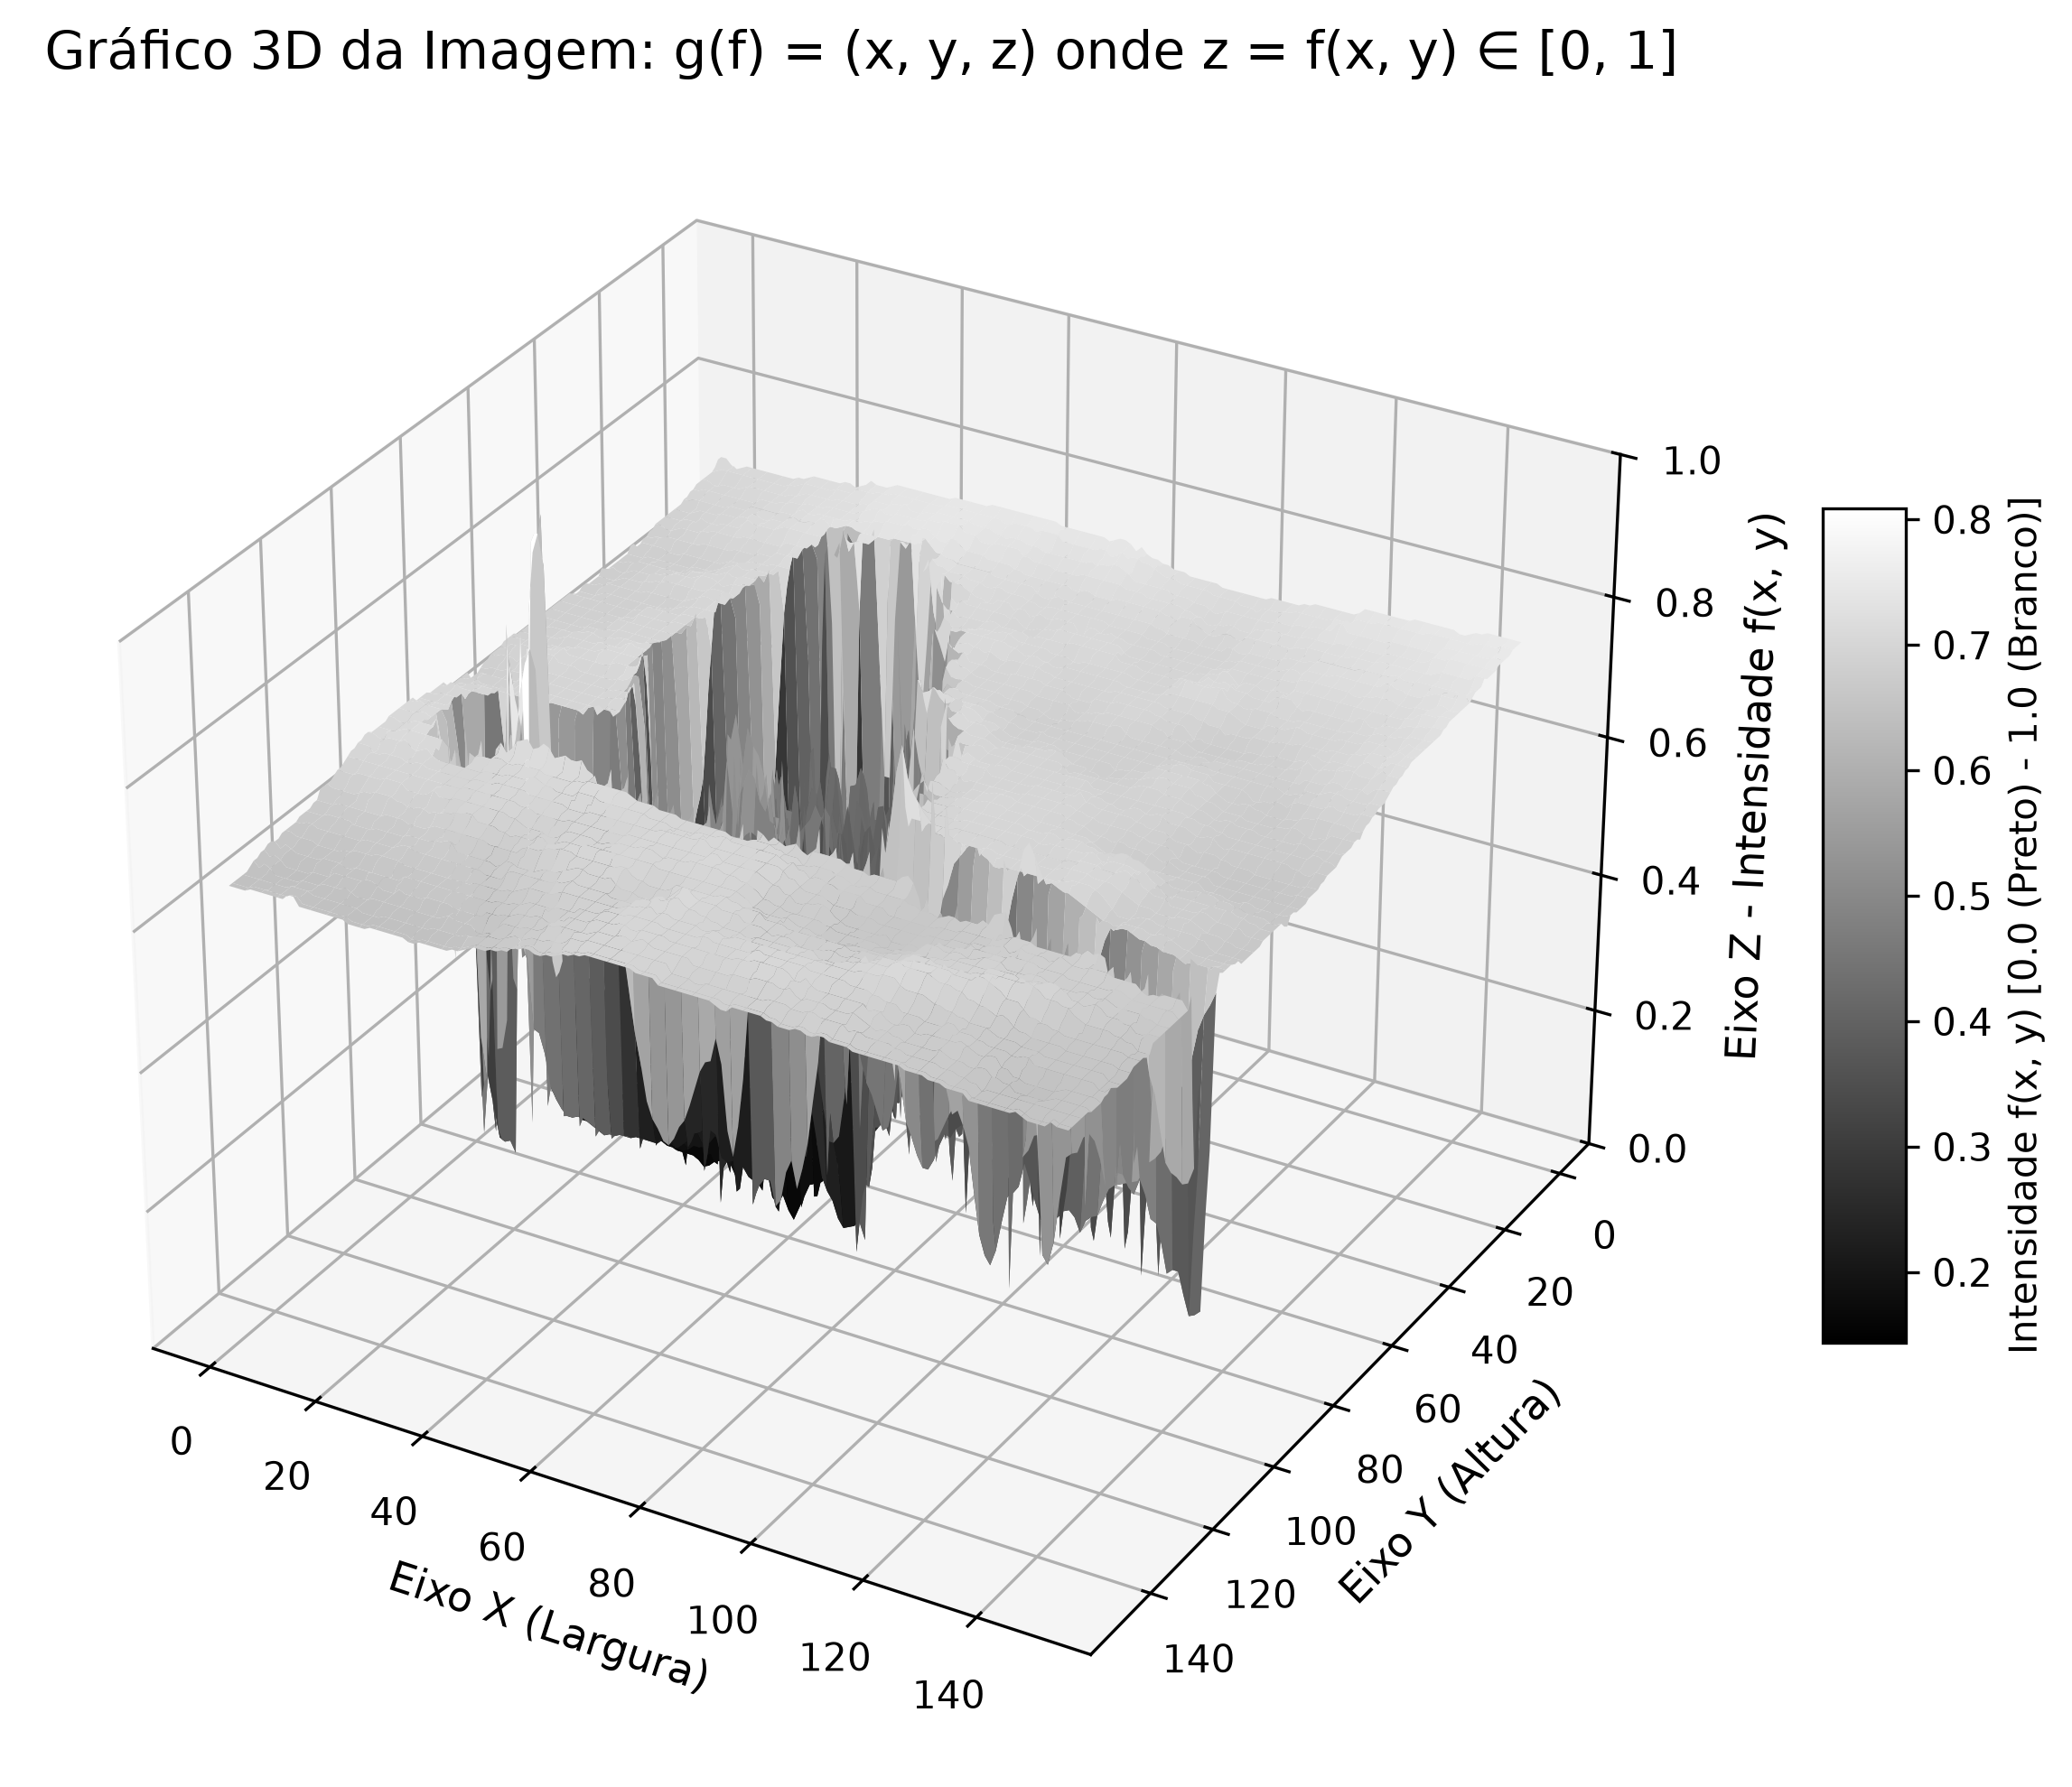
\includegraphics[width=0.5\linewidth]{grafico_imagem_3d.png}
	\caption{Representação tridimensional do gráfico $G(f)$ de uma imagem.}
	\label{fig:grafico_imagem}
\end{figure}

\section{Amostragem Espacial}

Para que uma imagem contínua $f: U \to V$ possa ser armazenada e processada digitalmente, é necessário discretizar tanto o domínio espacial $U \subset \mathbb{R}^2$ quanto o contradomínio de intensidades $V$. O processo de discretização do domínio espacial é denominado \textbf{amostragem}.

\begin{Defini}[Reticulado de Amostragem]
Seja $U = [a,b] \times [c,d] \subset \mathbb{R}^2$ o domínio contínuo da imagem. Para inteiros $M, N \ge 2$, definem-se os passos de amostragem uniforme nas direções $x$ e $y$, respectivamente, por:
\begin{equation}
\Delta x = \frac{b-a}{M-1} \quad \text{e} \quad \Delta y = \frac{d-c}{N-1}
\end{equation}
O \textbf{reticulado discreto de amostragem} é o subconjunto finito $\Lambda_{M,N} \subset U$ dado por:
\begin{equation}
\Lambda_{M,N} = \big\{ (x_m, y_n) \in U : x_m = a + m \Delta x, \; y_n = c + n \Delta y, \; m = 0, \dots, M-1, \; n = 0, \dots, N-1 \big\}
\end{equation}
\end{Defini}

A Figura \ref{fig:malha_bidimensional} ilustra a estrutura reticular de uma amostragem bidimensional sobre o domínio retangular.

\begin{figure}[H]
	\centering
	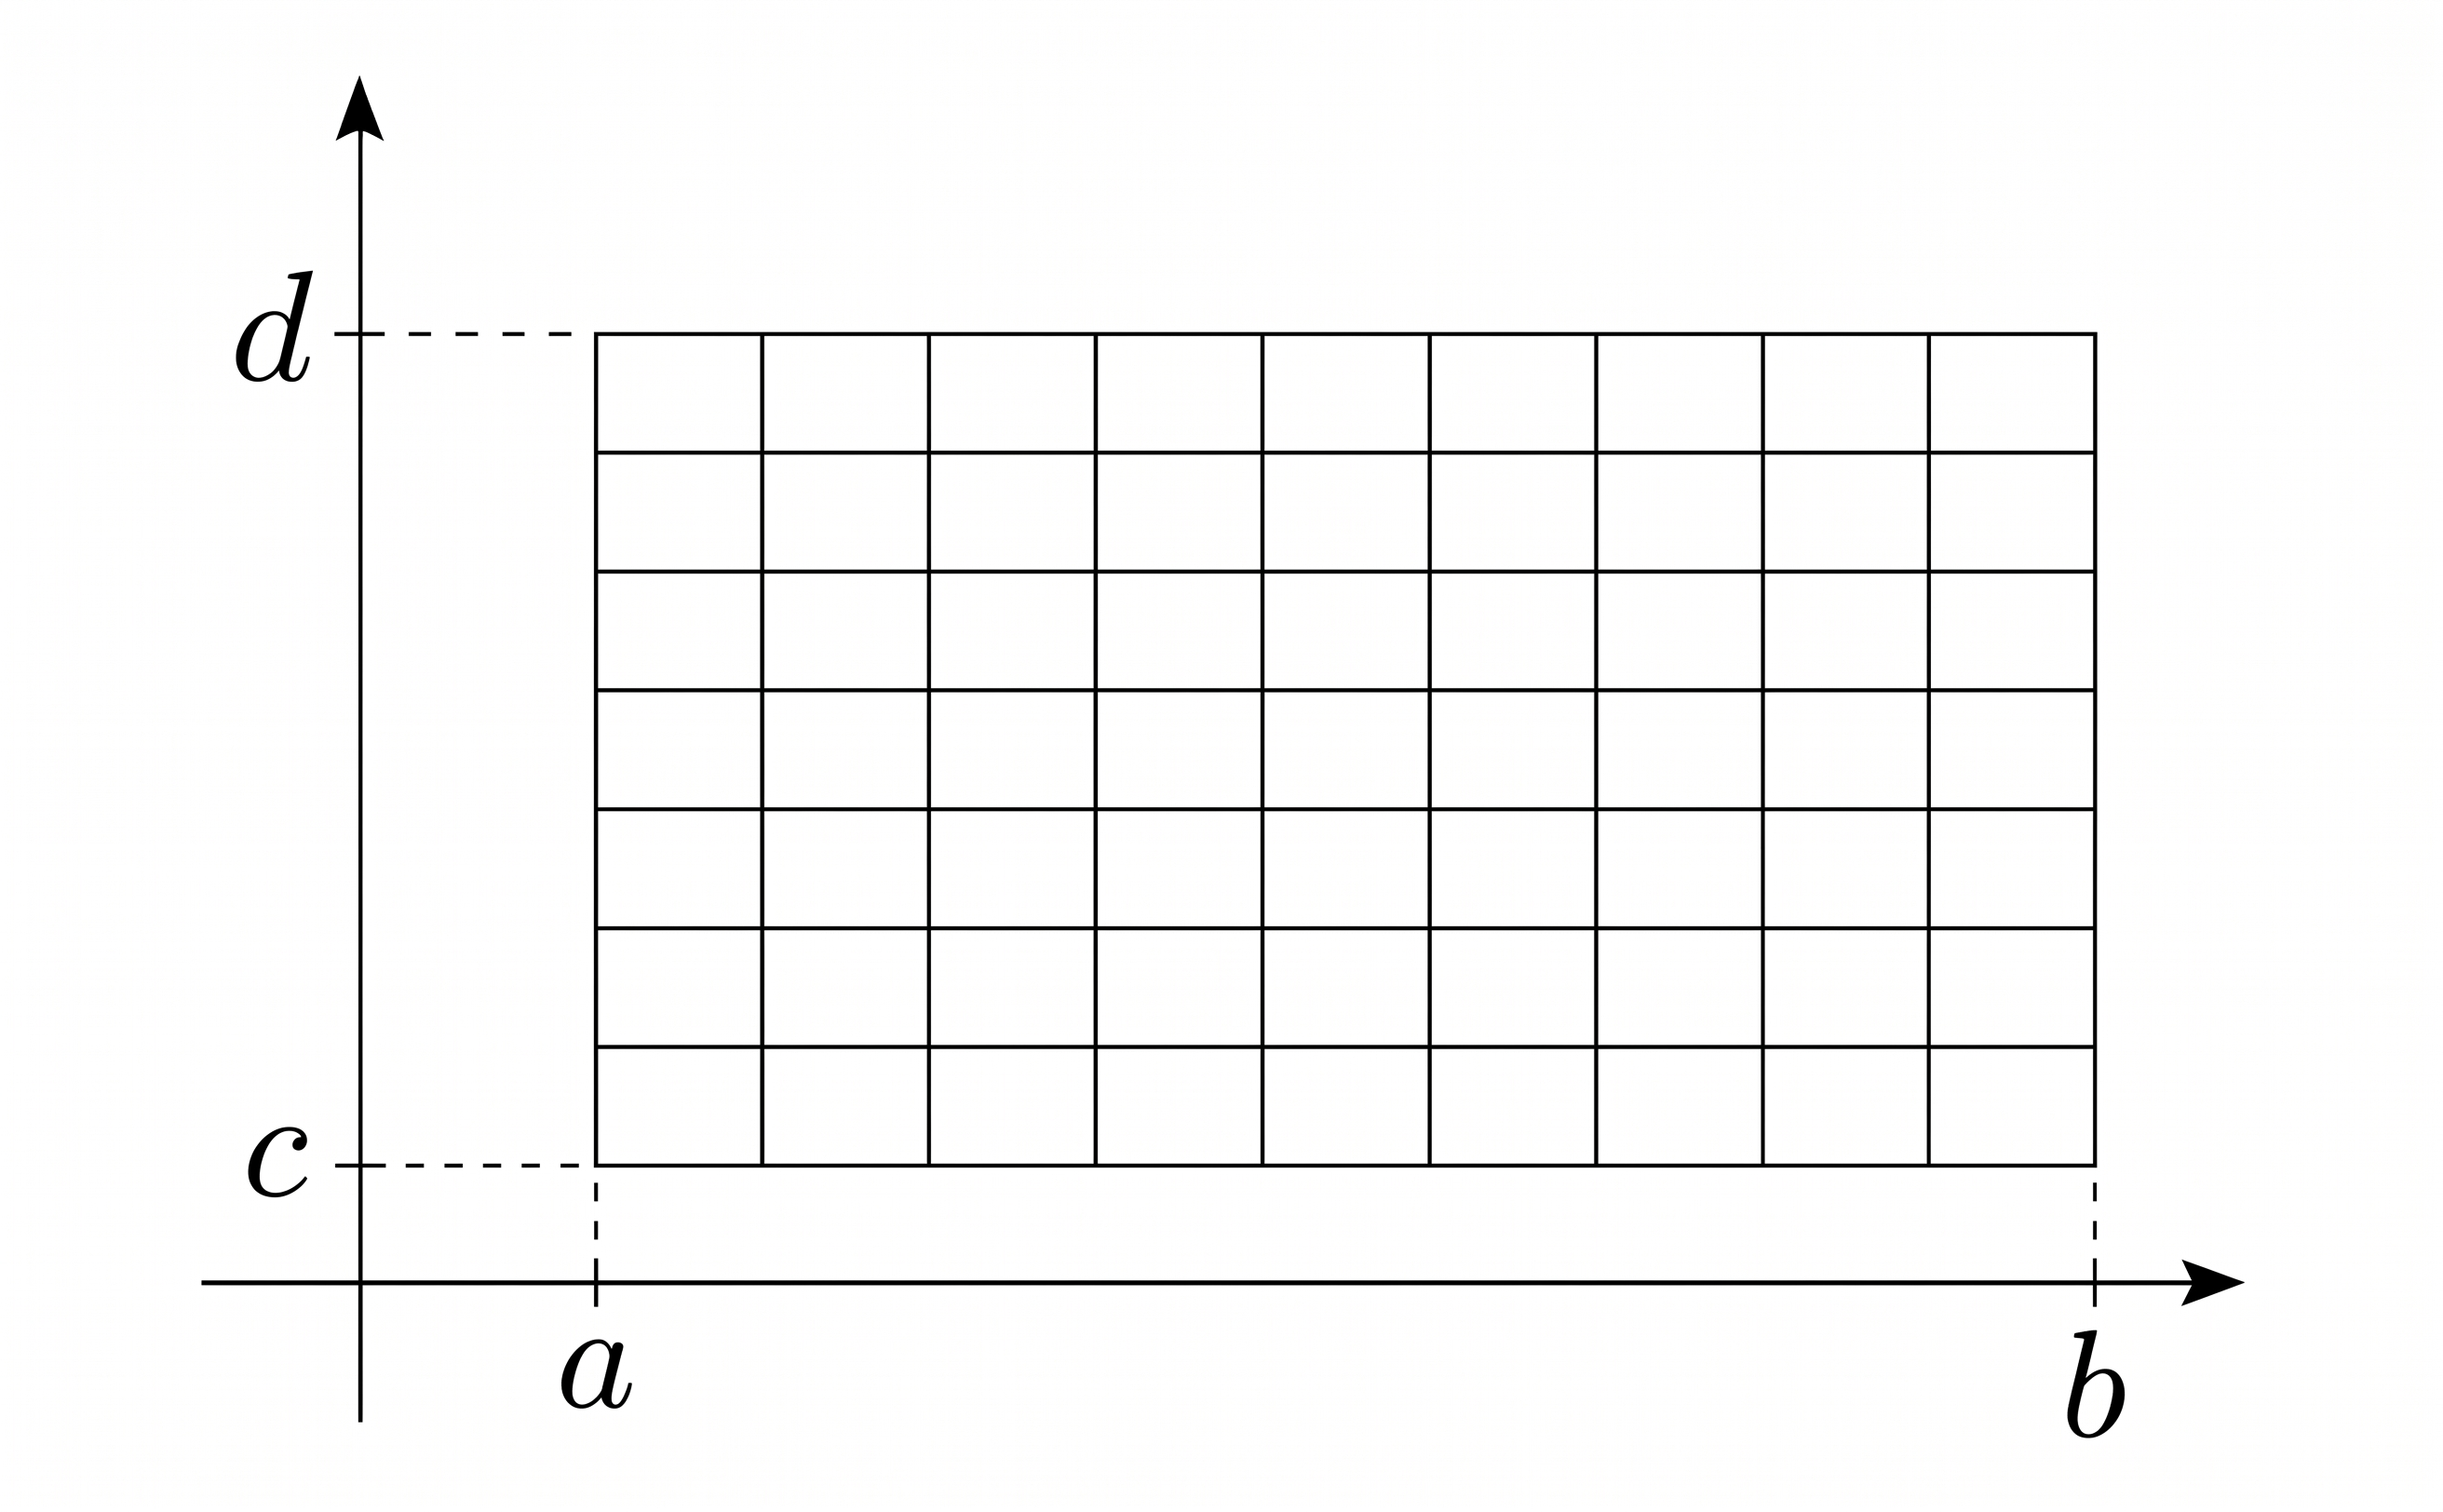
\includegraphics[width=0.5\linewidth]{malha_bidimensional.jpeg}
	\caption{Reticulado bidimensional de amostragem $\Lambda_{M,N}$.}
	\label{fig:malha_bidimensional}
\end{figure}

\begin{Defini}[Operadores de Amostragem]
Dada uma imagem contínua $f: U \to V$:
\begin{enumerate}[(i)]
	\item O \textbf{operador de amostragem ideal} $\mathcal{S}_{\text{ideal}}: \mathcal{F}(U, V) \to \mathcal{F}(\Lambda_{M,N}, V)$ avalia a função $f$ exatamente nos pontos do reticulado:
	\begin{equation}
	(\mathcal{S}_{\text{ideal}} f)(m,n) = f(x_m, y_n), \quad \forall (m,n) \in \{0, \dots, M-1\} \times \{0, \dots, N-1\}
	\end{equation}
	\item O \textbf{operador de amostragem por média integral} (modelo físico de integração em sensores CCD/CMOS) $\mathcal{S}_{\text{int}}: \mathcal{F}(U, V) \to \mathcal{F}(\Lambda_{M,N}, V)$ calcula a média espacial de $f$ sobre cada célula de amostragem $R_{m,n} \subset U$:
	\begin{equation}
	(\mathcal{S}_{\text{int}} f)(m,n) = \frac{1}{|R_{m,n}|} \iint_{R_{m,n}} f(x,y) \, dx \, dy
	\end{equation}
	onde $R_{m,n} = \left[x_m - \frac{\Delta x}{2}, x_m + \frac{\Delta x}{2}\right] \times \left[y_n - \frac{\Delta y}{2}, y_n + \frac{\Delta y}{2}\right]$ e $|R_{m,n}| = \Delta x \Delta y$.
\end{enumerate}
\end{Defini}

A amostragem estabelece a \textbf{resolução espacial} da imagem, definida pelo número de amostras $M \times N$. Cada elemento discreto da malha $(x_m, y_n)$ corresponde a um elemento de imagem, denominado \textit{picture element} ou \textbf{pixel}.

\section{Quantização de Intensidades}

Enquanto a amostragem discretiza o domínio espacial $U$, a \textbf{quantização} é o processo de discretização do contradomínio contínuo de intensidades $V = [L_{\min}, L_{\max}]$.

\begin{Defini}[Quantizador de Intensidade]
Seja $L \in \mathbb{N}$ ($L \ge 2$) o número de níveis discretos de intensidade. Uma \textbf{partição de quantização} de $V = [L_{\min}, L_{\max}]$ é uma coleção de $L+1$ limiares de decisão $\{t_0, t_1, \dots, t_L\}$ satisfazendo:
\begin{equation}
L_{\min} = t_0 < t_1 < t_2 < \dots < t_{L-1} < t_L = L_{\max}
\end{equation}
Estes limiares particionam $V$ nos subintervalos $I_k = [t_k, t_{k+1})$ para $k = 0, \dots, L-2$ e $I_{L-1} = [t_{L-1}, t_L]$.

Seja $\mathcal{Q} = \{q_0, q_1, \dots, q_{L-1}\} \subset V$ o conjunto dos \textbf{níveis de reconstrução} (representantes), tais que $q_k \in I_k$. O \textbf{operador de quantização} é a função degrau $Q: V \to \mathcal{Q}$ dada por:
\begin{equation}
Q(v) = q_k \quad \text{se } v \in I_k, \; k = 0, \dots, L-1
\end{equation}
\end{Defini}

\begin{Defini}[Quantização Uniforme]
A quantização diz-se \textbf{uniforme} se todos os subintervalos $I_k$ possuem a mesma amplitude $\Delta q > 0$:
\begin{equation}
\Delta q = \frac{L_{\max} - L_{\min}}{L}
\end{equation}
Nesse caso, os limiares de decisão são dados por $t_k = L_{\min} + k \Delta q$, e os representantes $q_k$ são usualmente fixados no ponto médio $q_k = L_{\min} + \left(k + \frac{1}{2}\right)\Delta q$.

Na prática computacional, mapeiam-se os níveis de intensidade para o conjunto discreto de inteiros $\{0, 1, \dots, L-1\}$ através da regra:
\begin{equation}
q(v) = \min \left\{ \left\lfloor \frac{v - L_{\min}}{\Delta q} \right\rfloor, \, L - 1 \right\} \in \{0, 1, \dots, L-1\}
\end{equation}
\end{Defini}

Em computação de imagens, o número de níveis $L$ é tipicamente uma potência de 2, isto é, $L = 2^k$, em que $k \in \mathbb{N}$ indica a quantidade de bits por pixel. Por exemplo, para $k=8$ bits, dispõe-se de $L = 256$ níveis discretos de cinza, indexados de $0$ (preto absoluto) a $255$ (branco absoluto).

\section{Imagem Digital e Representação Matricial}

A formalização da imagem digital decorre da aplicação conjunta dos operadores de amostragem e quantização.

\begin{Defini}[Imagem Digital]
Uma \textbf{imagem digital} é a função discreta $I: \{0, \dots, M-1\} \times \{0, \dots, N-1\} \to \mathcal{Q}$ obtida pela composição do operador de quantização $Q$ com o operador de amostragem $\mathcal{S}$ aplicados à imagem contínua $f: U \to V$:
\begin{equation}
I(m,n) = (Q \circ \mathcal{S} f)(m,n) = Q(f(x_m, y_n))
\end{equation}
Do ponto de vista da álgebra linear, a imagem digital $I$ é representada por uma matriz $M \times N$:
\begin{equation}
I = \begin{pmatrix}
I(0,0) & I(0,1) & \dots & I(0, N-1) \\
I(1,0) & I(1,1) & \dots & I(1, N-1) \\
\vdots & \vdots & \ddots & \vdots \\
I(M-1,0) & I(M-1,1) & \dots & I(M-1, N-1)
\end{pmatrix} \in \mathcal{M}_{M \times N}(\mathcal{Q})
\end{equation}
onde cada componente $I(m,n)$ armazena o nível de intensidade quantizado do pixel na linha $m$ e coluna $n$.
\end{Defini}

\subsection{Capacidade de Armazenamento}

A quantidade total de memória $b$ (em bits) requerida para armazenar uma imagem digital $M \times N$ não comprimida com $L = 2^k$ níveis de intensidade é dada por:
\begin{equation}
b = M \times N \times k = M \times N \times \log_2 L \quad \text{(bits)}
\end{equation}

\section{Reconstrução e Interpolação de Imagens}

A \textbf{interpolação} é o processo de estimar os valores de uma função contínua $\tilde{f}: U \subset \mathbb{R}^2 \to \mathbb{R}$ em pontos arbitrários do domínio a partir das amostras discretas $I(m,n)$ da imagem digital. Esse procedimento é essencial para operações de redimensionamento (zooming), rotação e deformações geométricas de imagens.

\subsection{Interpolação pelo Vizinho Mais Próximo}

Neste método, o valor atribuído a qualquer ponto $(x,y) \in U$ é igual ao nível de intensidade do pixel do reticulado $\Lambda_{M,N}$ geometricamente mais próximo de $(x,y)$.

\begin{Defini}[Interpolação pelo Vizinho Mais Próximo]
Dada a imagem digital $I$, a função interpolada pelo vizinho mais próximo $\tilde{f}_{\text{VP}}: U \to \mathbb{R}$ é dada por:
\begin{equation}
\tilde{f}_{\text{VP}}(x,y) = I(m^*, n^*), \quad \text{onde } (m^*, n^*) = \arg\min_{(m,n)} \sqrt{(x - x_m)^2 + (y - y_n)^2}
\end{equation}
\end{Defini}
A função $\tilde{f}_{\text{VP}}$ é constante por partes sobre as células do reticulado, resultando em descontinuidades visíveis conhecidas como efeito de blocos ou pixelização.

\subsection{Interpolação Bilinear}

Para obter uma reconstrução contínua $\tilde{f} \in C^0(U)$, aplica-se a interpolação bilinear utilizando os 4 vizinhos mais próximos.

\begin{Defini}[Interpolação Bilinear]
Para $(x,y) \in [x_m, x_{m+1}] \times [y_n, y_{n+1}] \subset U$, a função interpolante bilinear $\tilde{f}_{\text{bil}}$ é dada pela expressão polinomial:
\begin{equation}
\tilde{f}_{\text{bil}}(x,y) = a_0 + a_1 x + a_2 y + a_3 x y
\end{equation}
Os coeficientes reais $\{a_0, a_1, a_2, a_3\}$ são univocamente determinados exigindo-se que $\tilde{f}_{\text{bil}}$ coincida com a matriz de imagem nos 4 vértices da célula:
\begin{equation}
\tilde{f}_{\text{bil}}(x_i, y_j) = I(i,j), \quad \forall (i,j) \in \{(m,n), \, (m+1,n), \, (m,n+1), \, (m+1,n+1)\}
\end{equation}
\end{Defini}

\subsection{Interpolação Bicúbica}

A interpolação bicúbica produz uma superfície interpolante de classe $C^1(U)$, com derivadas parciais contínuas, preservando detalhes finos e atenuando serrilhados.

\begin{Defini}[Interpolação Bicúbica]
Para $(x,y) \in [x_m, x_{m+1}] \times [y_n, y_{n+1}]$, a função de interpolação bicúbica $\tilde{f}_{\text{bic}}$ utiliza os 16 pixels da vizinhança $4 \times 4$ em torno do ponto e assume a forma:
\begin{equation}
\tilde{f}_{\text{bic}}(x,y) = \sum_{i=0}^{3} \sum_{j=0}^{3} a_{ij} x^i y^j
\end{equation}
Os 16 coeficientes $\{a_{ij}\}$ são determinados ajustando o polinômio aos valores da imagem e às suas derivadas parciais ($\frac{\partial f}{\partial x}$, $\frac{\partial f}{\partial y}$, $\frac{\partial^2 f}{\partial x \partial y}$) estimadas nos vértices da célula.
\end{Defini}

\section{Vizinhança e Topologia Discreta no Reticulado}

No processamento digital de imagens, a análise de adjacência e conectividade entre pixels no reticulado discreto $\mathbb{Z}^2$ é fundamental para a definição de regiões, fronteiras e operadores morfológicos.

\begin{Defini}[Vizinhanças Discretas]
Seja $p = (m,n) \in \mathbb{Z}^2$ um pixel do reticulado:
\begin{enumerate}[(i)]
	\item A \textbf{4-vizinhança} de $p$, denotada por $N_4(p)$, é o conjunto dos 4 pixels ortogonalmente adjacentes a $p$:
	\begin{equation}
	N_4(p) = \big\{ (m+1, n), \, (m-1, n), \, (m, n+1), \, (m, n-1) \big\}
	\end{equation}
	\item A \textbf{vizinhança diagonal} de $p$, denotada por $N_D(p)$, é o conjunto dos 4 pixels diagonalmente adjacentes a $p$:
	\begin{equation}
	N_D(p) = \big\{ (m+1, n+1), \, (m+1, n-1), \, (m-1, n+1), \, (m-1, n-1) \big\}
	\end{equation}
	\item A \textbf{8-vizinhança} de $p$, denotada por $N_8(p)$, é a união da 4-vizinhança com a vizinhança diagonal:
	\begin{equation}
	N_8(p) = N_4(p) \cup N_D(p)
	\end{equation}
\end{enumerate}
\end{Defini}
	
	
	
	
	
	\newpage
	
	%%%%%%%%%%%%%%%%%%%%%%%%%%%%%%%%%%%%%%
	
	\chapter{O Teorema de Ascoli-Arzelá}
	
	
	\newpage
	
	%%%%%%%%%%%%%%%%%%%%%%%%%%%%%%%%%%%%%%
	
	\chapter{Aplicações}
	
	
	
	\newpage
	
	%%%%%%%%%%%%%%%%%%%%%%%%%%%%%%%%%%%%%%
	
	\chapter*{Conclusão}
	\addcontentsline{toc}{chapter}{Conclusão}
	
	
	
	
	\newpage
	
	%%%%%%%%%%%%%%%%%%%%%%%%%%%%%%%%%%%%%%%
	
	\begin{thebibliography}{99}
		\addcontentsline{toc}{chapter}{Referências Bibliográficas}
		
		\bibitem{Geraldo} ÁVILA, Geraldo Severo de Souza. Introdução à Análise Matemática. 2. ed. São Paulo: Blucher, 1999.
		
		\bibitem{edo} DOERING, Claus Ivo; LOPES, Artur Oscar. Equações Diferenciais Ordinárias. 6. ed. Rio de Janeiro: IMPA, 2016. 
		
		\bibitem{fino} LIMA, Elon Lages. Análise real volume 1. Funções de uma variável. 12. ed. Rio de Janeiro: IMPA, 2017.
		
		\bibitem{Elon} LIMA, Elon Lages. Curso de Análise. 14. ed. Rio de Janeiro: IMPA, 1976. v. 1. 
		
		\bibitem{rn} LIMA, Elon Lages. Curso de Análise, Volume 2. Rio de Janeiro: IMPA, 1999.
		
		\bibitem{metricos} LIMA, Elon Lages. Espaços Métricos. 5. ed. Rio de Janeiro: IMPA, 2017.
		
		\bibitem{historia} EVES, Howard. Introdução à história da matemática / Howard Eves; tradução Hygino H. Domingues. 5a ed. - Campinas, SP: Editora da Unicamp, 2011.
		
		\bibitem{Neri} NERI, Cassio; CABRAL, Marco. Curso de Análise Real. 1. ed. Rio de Janeiro.
		
		
		
	\end{thebibliography}
	
	
	\newpage
	
	
	
	
	
\end{document}
